\chapter{Sample Exam Paper 2}
\section{Question 1}
\textit{A car factory makes 850,000 cars per year. Each car takes four 8-hour days of direct labour at the rate of \pounds 21 per hour. Overhead costs are estimated at \pounds 11 per direct labour hour. A new production process would reduce the direct labour per car by 25\%, but increase overhead costs by 20\% per direct labour hour. If all other costs remain the same, what is the maximum amount of money you would pay for this new process? Assume that the new process must pay for itself by the end of the first year. .}

\textbf{5 marks}

Old process:
\begin{gather}
    850000\times 32\times \left(21+11\right) = \SI{870400000}{\pounds}
\end{gather}
New process:
\begin{gather}
    850000\times 24 \times \left(21+13.2\right) = \SI{697680000}{\pounds}
\end{gather}
Maximum amount that should be paid:
\begin{gather}
    \SI{870400000}{\pounds} - \SI{697680000}{\pounds} = \SI{172720000}{\pounds}
\end{gather}
\section{Question 2}
\textit{A manufacturer is deciding whether or not to purchase a new piece of equipment. Uncertain market conditions mean that the capital costs and annual benefits associated with this piece of equipment are uncertain (see Table \ref{tab:capCostsQ2}). The useful life of the equipment is three years. Assume that MARR=10\% and the market value at the end of its useful life is zero. }

\textbf{25 marks}

\begin{table}[H]
    \centering
    \begin{tabular}{@{}lll@{}}
        \toprule
        \textbf{Capital costs (\pounds)} & \textbf{Annual benefits (\pounds)} & \textbf{Probability of outcome} \\
        \midrule
        300,000                          & 120,000                            & 0.1                             \\
        500,000                          & 200,000                            & 0.3                             \\
        400,000                          & 150,000                            & 0.6                             \\
        \bottomrule
    \end{tabular}
    \caption{Potential capital costs and benefits of the equipment for Question 2.}
    \label{tab:capCostsQ2}
\end{table}
\textit{What is the average NPV?}

\textbf{25 marks}
\begin{gather}
    -300000+120000\times \frac{1.1^3-1}{0.1\times 1.1^3} = \SI{-1577.76}{\pounds}\\
    -500000+200000\times frac{1.1^3-1}{0.1\times 1.1^3} = \SI{-2629.60}{\pounds}\\
    -500000+150000\times frac{1.1^3-1}{0.1\times 1.1^3} = \SI{-26972.20}{\pounds}\\
    E\left(NPV\right) = \left(-1577.76\times 0.1\right) + \left(-2629.60\times 0.3\right) + \left(-26972.20\times 0.6\right) = \SI{-17129.98}{\pounds}
\end{gather}
\textit{What is the probability that the decision to buy the piece of equipment is a good one?}

\textbf{5 marks}
\begin{gather}
    P\left(NPV > 0\right) = 0
\end{gather}
No outcomes give a positive NPV value, therefore buying the equipment is not a good choice in any case.
\section{Question 3}
\textit{A firm must decide between constructing a new facility or renting office space to accommodate the expected growth of this company over the next 10 years (see Figure \ref{fig:dt2}).}

\textit{If the company opts to construct a new facility, additional space may be required in five years (the probability of this occurring can be worked out from other probabilities provided in the tree), depending on its size. If additional space is required, there will be an option to build an office addition or rent space for the additional space requirements. If additional space is not required, operating and maintenance costs will be larger than \pounds 200,000 per year in the first five years.}

\textit{MARR is 10\% per year. An NPV analysis is to be conducted on the alternatives. Which course of action should be recommended? }

\textbf{30 marks}
\begin{figure}[H]
    \centering
    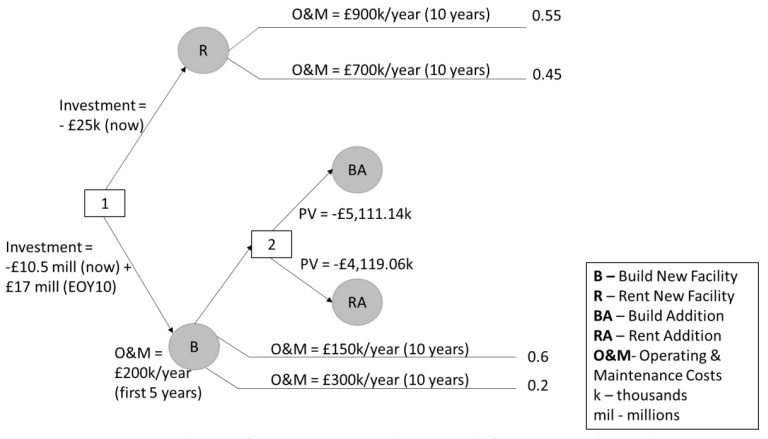
\includegraphics[width = 0.9\textwidth]{img/figure68.png}
    \caption{Decision tree for Question 3. EOY denotes end-of-year and PV denotes the net present value associated with the alternative.}
    \label{fig:dt2}
\end{figure}
Consider the renting option:
\begin{align}
    (1) & -25000-900000\times \frac{1.1^10-1}{0.1\times 1.1^10} = \SI{-5555110.40}{\pounds} & p(1) = 0.55 \\
    (2) & -25000-700000\times \frac{1.1^10-1}{0.1\times 1.1^10} = \SI{-4326196.97}{\pounds} & p(2) = 0.45
\end{align}
Therefore average NPV for renting is:
\begin{gather}
    E(NPV_{\textrm{renting}}) = \left(0.55\times-5555110.40\right) + \left(0.45\times-4326196.97\right) = \SI{-5002099.36}{\pounds}
\end{gather}
Consider the building option and additional space is required (we choose rent addition as build addition is more expensive and eliminated from consideration):
\begin{align}
    (1) & -10500000 - 200000\times \frac{1.1^5-1}{0.1\times 1.1^5} -4119060 +\frac{17000000}{1.1^{10}} = \SI{-8822981.43}{\pounds} & p(1) = 0.2
\end{align}
Consider the buying option and no additional space is required:
\begin{align}
    (2) & -10500000 - 200000\times \frac{1.1^5-1}{0.1\times 1.1^5} - 150000\times \frac{1.1^{10} - 1}{0.1\times 1.1^{10}} +\frac{17000000}{1.1^{10}} = \SI{-5625606.50}{\pounds} & p(2) = 0.6 \\
    (3) & -10500000 - 200000\times \frac{1.1^5-1}{0.1\times 1.1^5} - 300000\times \frac{1.1^{10} - 1}{0.1\times 1.1^{10}} +\frac{17000000}{1.1^{10}} = \SI{-6547291.57}{\pounds} & p(3) = 0.2
\end{align}
Therefore average NPV for building is:
\begin{multline}
    E(NPV_{\textrm{building}}) = \left(0.2\times-8822981.43\right) + \left(0.6\times-5625606.50\right) + \left(0.2\times-6547291.57\right) = \SI{-6449418.5}{\pounds}
\end{multline}
Average NPV for renting is lower than the average NPV for building, hence it should be recommended to rent office space to accommodate growth.
\section{Question 4}
UCL Engineering plc is a multinational engineering equipment trader and distribution company that has been established for many years. Its income and balance sheet for two years are provided in Table \ref{tab:incStat2} and Table \ref{tab:balSheet2} respectively.
\begin{table}[H]
    \centering
    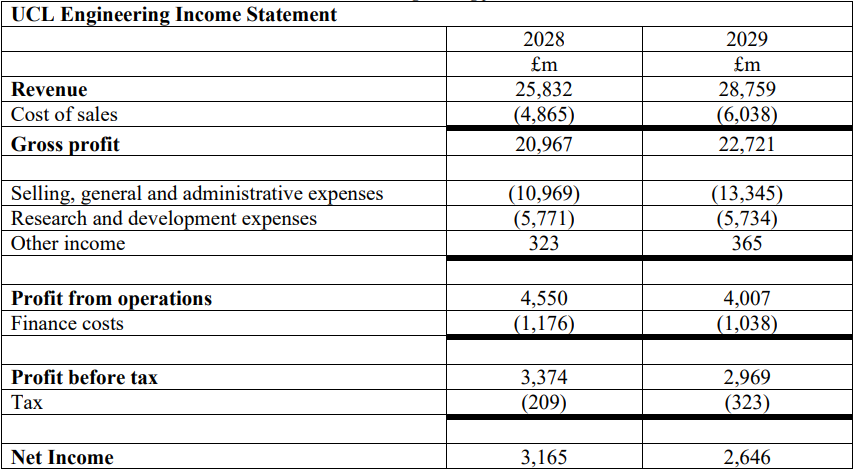
\includegraphics[width = 0.9\textwidth]{img/figure69.png}
    \caption{UCL Engineering plc income statement.}
    \label{tab:incStat2}
\end{table}
\begin{table}[H]
    \centering
    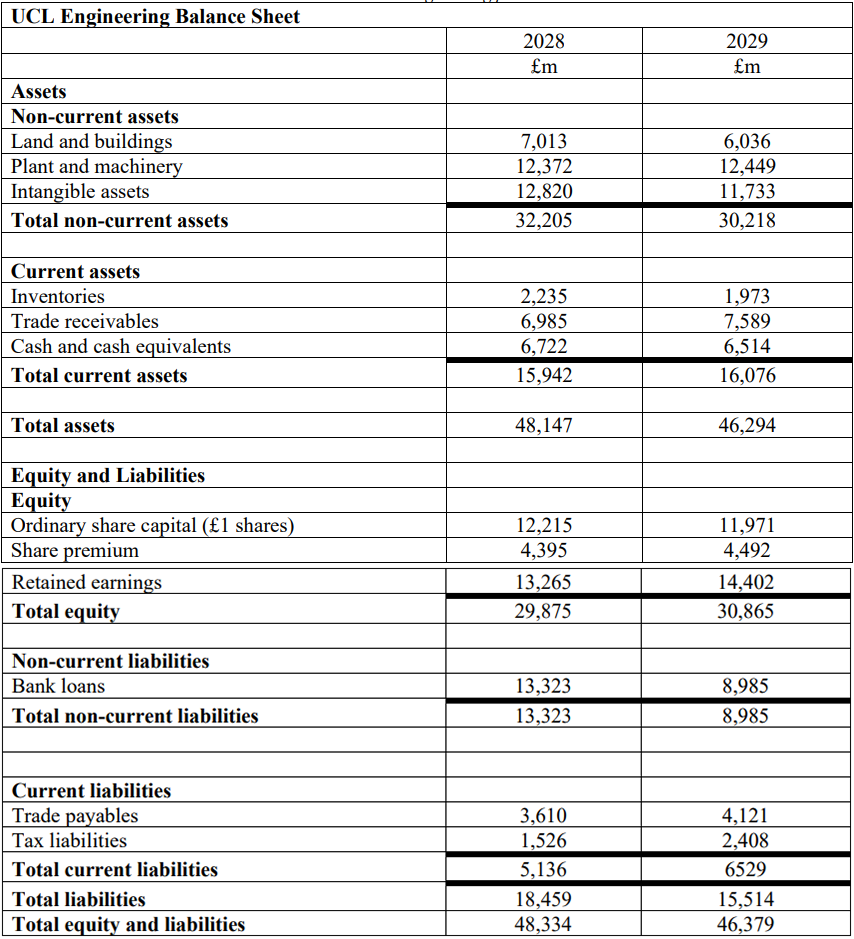
\includegraphics[width = 0.7\textwidth]{img/figure70.png}
    \caption{UCL Engineering plc balance sheet.  Note the inventory for the company in 2027 is valued at \pounds 2,350 million.}
    \label{tab:balSheet2}
\end{table}
\textit{Explain the terms ``net income'', ``intangible assets'' and ``equity'' that feature in either the Income Statement or the Balance Sheet.}

\textbf{10 marks}
\begin{itemize}
    \item Net income is the amount of profit left after all expenses have been paid.
    \item Intangible assets are assets that are not physical in nature. They are a type of non-current asset meaning that they are not expected to be converted to cash over the next one-year period.
    \item Equity is what the company owes to shareholders and is what remains of the assets after all liabilities have been paid.
\end{itemize}
\textit{Calculate the financial ratios shown in Table \ref{tab:finRatio2} and use them to provide a one-paragraph interpretation of the company's general performance.}

\textbf{30 marks}
\begin{table}[H]
    \centering
    \begin{tabular}{@{}lcccc@{}}
        \toprule
                                   & \textbf{Formula}                                                & \textbf{2028}                 & \textbf{2029}                 & \textbf{Industry average} \\
        \midrule
        \addlinespace[0.5em]
        Current ratio              & $\dfrac{\textrm{Current assets}}{\textrm{Current liabilities}}$ & $\dfrac{15942}{5136} = 3.10$  & $\dfrac{16076}{6529} = 2.46$  & 2.4                       \\
        \addlinespace[1em]
        Debt-Equity ratio          & $\dfrac{\textrm{Total liabilities}}{\textrm{Total equity}}$     & $\dfrac{18459}{29875} = 0.62$ & $\dfrac{15514}{30865} = 0.50$ & 38.38\%                   \\
        \addlinespace[1em]
        Total asset turnover ratio & $\dfrac{\textrm{Total annual sales}}{\textrm{Total assets}}$    & $\dfrac{25832}{48147} = 0.54$ & $\dfrac{28759}{46294} = 0.62$ & 0.85                      \\
        \addlinespace[1em]
        Profit margin              & $\dfrac{\textrm{Net income}}{\textrm{Net sales}}$               & $\dfrac{3165}{25832} = 0.12$  & $\dfrac{2646}{22721} = 0.09$  & 8.5\%                     \\
        \addlinespace[0.5em]
        \bottomrule
    \end{tabular}
    \caption{Financial ratios and their industry average values for Question 4.}
    \label{tab:finRatio2}
\end{table}
Compared to industry averages, the company demonstrates a variety of strengths and shortcomings in its financial performance. The company's liquidity is robust, outpacing the high industry standard with a current ratio of 3.10 in 2028 and 2.46 in 2029, exceeding the industry average of 2.4. Conversely, the company embodies a higher risk to shareholders than the industry standard, with a debt-equity ratio of 0.62 in 2028 and 0.50 in 2029, surpassing the average of 38.38\%.

In terms of profitability, the company markedly surpassed the industry average in 2028. Although the profit margin of 9\% in 2029 is only slightly above the industry average of 8.5\%, it suggests a continuation of the prior year's performance. However, in both 2028 and 2029, the company underperformed the industry average in utilising assets to generate sales, as indicated by the total asset turnover ratio of 0.54 and 0.62, respectively, falling short of the industry average of 0.85.

Inter-year comparison of these ratios presents a discernible trend. The company's liquidity is generally declining, as shown by the decreasing current ratio from 2028 to 2029. Despite this, the company is becoming less risky for shareholders, evidenced by the reduced debt-equity ratio. Furthermore, there is an indication of improving efficiency in asset utilisation, given the increase in the total asset turnover ratio. Nonetheless, there is a general downtrend in profitability, with the profit margin declining from 2028 to 2029.